\chapter{Selection Efficiencies and Purities, 2017}
\label{chap:eff_2017}
This chapter presents on the efficiencies and purities of the 2017 ND280 analysis, summarised in \autoref{tab:eff_pur_summary}.

\section{$\nu_\mu$ in FHC}
Using the aforementioned cuts we can study the lepton tagging efficiency and purity of each ND280 \numu selection. The number of events are the raw number of generated Monte-Carlo events without any weighting applied. We show the efficiencies as a function of reconstructed lepton candidate momentum, $p_{reco}$.

\autoref{fig:cc0pi_topology} shows the topology purity for the CC0$\pi$ selection in FGD1 and FGD2. The purity peak coincides with the event peak with $\sim85\%$ efficiency and falls off in both directions. The true CC$1\pi$ and CCOther topology constitute the selection very similarly, at about $10\%$ across the momentum range. As we move up in momentum the CC DIS cross-sections---the largest contribution to the CCOther final state---increase whilst the CCQE and 2p2h cross-sections---the largest contributions to the CC0$\pi$ final state---decrease. CC1$\pi$ and CC DIS interactions can produce low-momentum pions which aren't reconstructed in the detector and CC DIS can produce a $\pi^-$ which may be mistaken for the lepton candidate. Furthermore, the pions can undergo secondary interactions after exiting the nucleus, causing them to be undetected. The NC contribution comes primarily from the NC$1\pi^-$ via resonance interaction, in which the $\pi^-$ is identified as the lepton candidate and there are no other particles in the final state. We also note barely any anti-neutrino contamination, owing to the sign selection from the magnet, the low \numubar flux in FHC and the smaller cross-section. Averaging over the entire range we have purity of $75.5\%$ for FGD1 and $73.5\%$ for FGD2.
\begin{figure}[h]
	\begin{subfigure}[t]{0.49\textwidth}
		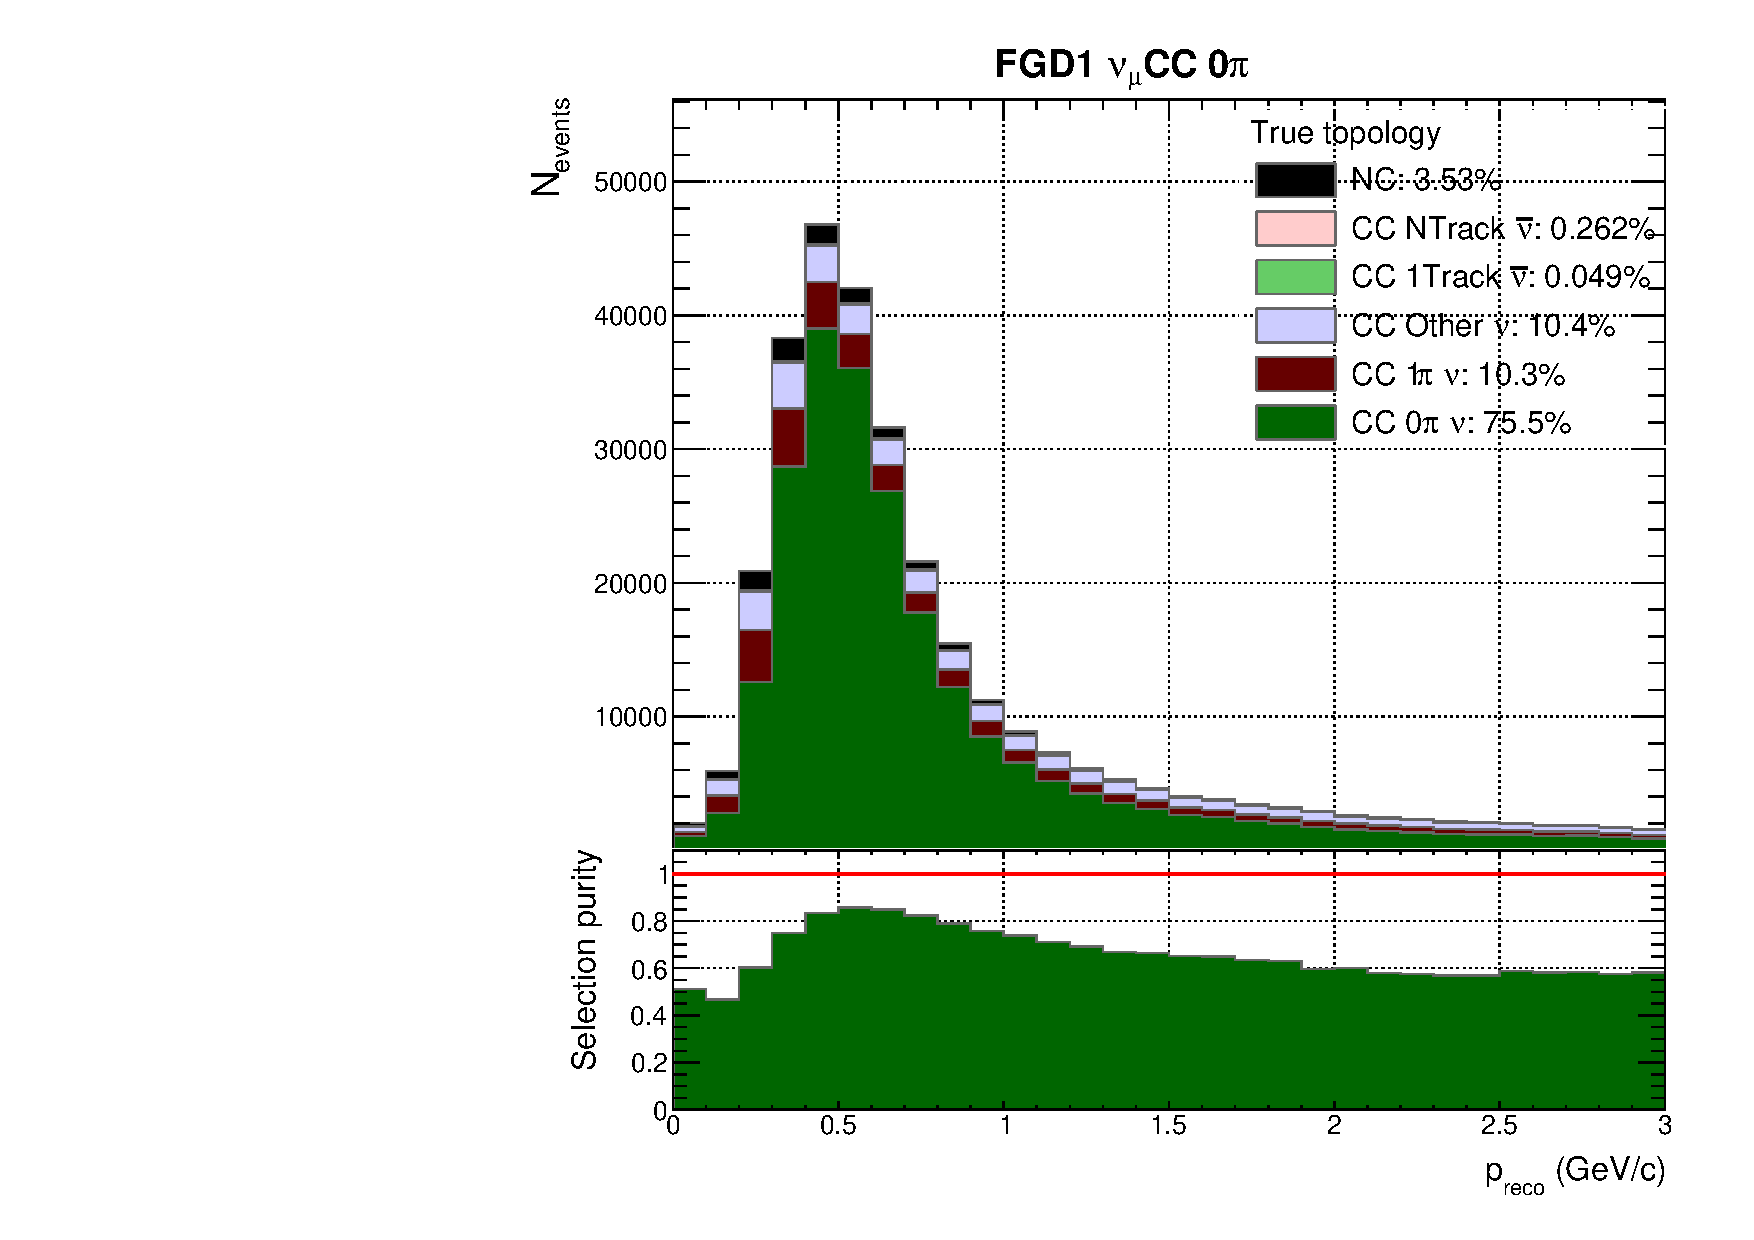
\includegraphics[width=\textwidth,page=1, trim={0mm 0mm 0mm 9mm}, clip]{figures/mach3/selection/2017b_Diag_WithSelection}
		\caption{FGD1}
	\end{subfigure}
	\begin{subfigure}[t]{0.49\textwidth}
		\includegraphics[width=\textwidth,page=7, trim={0mm 0mm 0mm 9mm}, clip]{figures/mach3/selection/2017b_Diag_WithSelection}
		\caption{FGD2}
	\end{subfigure}
	\caption{Breakdown of CC0$\pi$ selection events' true event topology for FGD1 and FGD2 }
	\label{fig:cc0pi_topology}
\end{figure}

\autoref{fig:cc0pi_muon} shows the muon tagging efficiency. We observe good performance over the range of muon momentum, starting with $\sim65\%$ at low momentum, plateauing at $\sim95\%$ above 500 MeV/c for both FGD1 and FGD2, which is where the majority of events reside. Averaging over the entire range, the muon tagging performance is 93.8\% for FGD1 and 93.2\% for FGD2. The largest background is $\pi^-$ from CC$1\pi$, CCOther and NC interactions, in which the $\pi^-$ is either created at the interaction vertex---e.g. an NC$1\pi^-$ via a resonance where there is no $\mu^-$, or a CCOther interaction creating multiple pions in which one $\pi^-$ has a higher reconstructed momentum than the $\mu^-$---or through final-state-interactions (FSI) in which a nucleon, $\pi^0$ or $\pi^+$ undergoes scattering on nucleons in the nucleus to produce the $\pi^-$.
\begin{figure}[h]
	\begin{subfigure}[t]{0.49\textwidth}
		\includegraphics[width=\textwidth,page=2, trim={0mm 0mm 0mm 9mm}, clip]{figures/mach3/selection/2017b_Diag_WithSelection}
		\caption{FGD1}
	\end{subfigure}
	\begin{subfigure}[t]{0.49\textwidth}
		\includegraphics[width=\textwidth,page=8, trim={0mm 0mm 0mm 9mm}, clip]{figures/mach3/selection/2017b_Diag_WithSelection}
		\caption{FGD2}
	\end{subfigure}
	\caption{Breakdown of selection CC0$\pi$ events' true lepton candidate for FGD1 and FGD2 }
	\label{fig:cc0pi_muon}
\end{figure}

\autoref{fig:cc1pi_topology} shows the topology purity for the CC1$\pi$ selection. Owing to identifying one single $\pi^+$ and one single $\pi^-$, the purity is notably worse for CC1$\pi$ compared to CC0$\pi$ and peaks at $p_{reco}\sim0.4\text{ GeV/c}$ with $\sim70\%$ purity. The purity takes the biggest hit from CCOther feed-down at $25\%$, in which either the lepton candidate is identified as a $\pi^-$ with an accompanying $\pi^+$, or events with a \{$\mu^-$, $\pi^+$, $\pi^{-,0}$\} have the latter pion unreconstructed from high-angle and low momentum tracks, leading to a poorly determined PID. The CCOther feed-down increases with $p_{reco}$ as the CC DIS cross-section increases: the main cause of the decreasing purity with increase $p_{reco}$. The CC0$\pi$ contributions comes from the outgoing proton being reconstructed as a $\pi^+$, or when the nucleon rescatters after exiting the nucleus, producing a pion-like track that gets associated with the primary vertex by mistake. The CC0$\pi$ contribution is concentrated in the first momentum bin, in which it makes up $\sim50\%$. The NC topology contributes 7\% by producing a \{$\pi^-$, $\pi^+$\} state through NC DIS or NC1$\pi$ with FSI which gets reconstructed as the \{$\mu^-$, $\pi^+$\} final state. The purity for CC1$\pi$ across the full momentum range is $58\%$ and very similar for FGD1 and FGD2.
\begin{figure}[h]
	\begin{subfigure}[t]{0.49\textwidth}
		\includegraphics[width=\textwidth,page=3, trim={0mm 0mm 0mm 9mm}, clip]{figures/mach3/selection/2017b_Diag_WithSelection}
		\caption{FGD1}
	\end{subfigure}
	\begin{subfigure}[t]{0.49\textwidth}
		\includegraphics[width=\textwidth,page=9, trim={0mm 0mm 0mm 9mm}, clip]{figures/mach3/selection/2017b_Diag_WithSelection}
		\caption{FGD2}
	\end{subfigure}
	\caption{Breakdown of selection CC1$\pi$ events' true event topology for FGD1 and FGD2 }
	\label{fig:cc1pi_topology}
\end{figure}

\autoref{fig:cc1pi_muon} shows the muon tagging efficiency for CC1$\pi^+$. As for the purity, the efficiency is comparably worse due to the additional pion requirement, averaging at 83\% across the $p_{reco}$ range. Common with the CC0$\pi$ efficiency in \autoref{fig:cc0pi_muon} the major background is $\pi^-$, which now constitutes 11\% instead of 4\%. The $\pi^-$ comes primarily from DIS interactions and CC1$\pi^0$ via resonances in which the $\pi^0$ undergoes a charge-exchange FSI, as discussed earlier. The $\pi^+$ contribution comes from high momentum pions which do not bend sufficiently to get a good PID: since the initial CC-inclusive search is done based on highest-momentum track this track is selected as the lepton candidate which curves similarly to a high-momentum $\mu^-$. As $p_{reco}$ increases the efficiency tends to similar values as the CC0$\pi$ selection.
\begin{figure}[h]
	\begin{subfigure}[t]{0.49\textwidth}
		\includegraphics[width=\textwidth,page=4, trim={0mm 0mm 0mm 9mm}, clip]{figures/mach3/selection/2017b_Diag_WithSelection}
		\caption{FGD1}
	\end{subfigure}
	\begin{subfigure}[t]{0.49\textwidth}
		\includegraphics[width=\textwidth,page=10, trim={0mm 0mm 0mm 9mm}, clip]{figures/mach3/selection/2017b_Diag_WithSelection}
		\caption{FGD2}
	\end{subfigure}
	\caption{Breakdown of selection CC1$\pi$ events' true lepton candidate for FGD1 and FGD2 }
	\label{fig:cc1pi_muon}
\end{figure}

\autoref{fig:ccoth_topology} shows the topology purity for the CCOther selection. As expected from the other purities, CCOther increases with $p_{reco}$ due to the increase in the CC DIS cross-section. The CC0$\pi$ and CC1$\pi$ topology seeps in to this selection by creating $\pi^{\pm,0}$ after exiting the nucleus that become(s) wrongly associated with the primary interaction vertex, or by the reconstruction falsely identifying an outgoing proton as a $\pi^+$. In the NC case, it is enough to have a interaction which produces a \{$\pi^-, \pi^0$\} combination, which can happen directly through NC DIS or indirectly with NC$1\pi$ via resonances, in which a secondary interaction occurs and the new track gets wrongly associated to the primary vertex. Initially, the purity starts at 35-40\% and plateaus around 80\% at $p_{reco} \sim 1.5\text{ GeV/c}$. Overall, the purity of the selection is 65\% for both FGDs over the entire range, with $\sim10\%$ each from NC, CC0$\pi$ and CC1$\pi$.
\begin{figure}[h]
	\begin{subfigure}[t]{0.49\textwidth}
		\includegraphics[width=\textwidth,page=5, trim={0mm 0mm 0mm 9mm}, clip]{figures/mach3/selection/2017b_Diag_WithSelection}
		\caption{FGD1}
	\end{subfigure}
	\begin{subfigure}[t]{0.49\textwidth}
		\includegraphics[width=\textwidth,page=11, trim={0mm 0mm 0mm 9mm}, clip]{figures/mach3/selection/2017b_Diag_WithSelection}
		\caption{FGD2}
	\end{subfigure}
	\caption{Breakdown of selection CCOther events' true event topology for FGD1 and FGD2 }
	\label{fig:ccoth_topology}
\end{figure}

\autoref{fig:ccoth_muon} shows the muon tag efficiency for the CC Other sample, which is notably worse than for previous selections: on average 73\%. This is expected, since the CCOther selection has at least 2 tracks (1$\mu^-$, 1$\pi^{\pm}$, 1$\pi^0$) but often even more. It is sufficient to have an interaction in which $N_\pi \ge 2$ and $p_{\pi} > p_{\mu}$ to wrongly identify the lepton candidate. Owing to the many tracks in this topology due to the CC and NC DIS interaction, it is no surprise to see a 20\% contribution from $\pi^-$. Furthermore, at low $p_{reco}$ electrons are selected a majority of the time, coming from two sources: 1) relatively high threshold of \numu CC DIS compared to \nue CC DIS due to the muon mass (even though the \nue flux is much lower than \numu) and 2) since the CCOther topology is the only topology to allow for $\pi^0$, these are likely to produce $e^\pm$ pairs in the TPC. If the $\pi^0$ shower occurs early in the TPC and the interaction vertex is traced to a downstream layer of the FGD, the electron may be falsely associated with the interaction vertex, and if $p_e > p_\mu$ is picked as the highest momentum candidate. To pass the TPC $\mu$ PID cut we would require a low momentum $e^-$ to match the dE/dx of a $\mu^-$, which in \autoref{fig:TPC_dedx} happens at $p\sim100\text{ MeV/c}$.
\begin{figure}[h]
	\begin{subfigure}[t]{0.49\textwidth}
		\includegraphics[width=\textwidth,page=6, trim={0mm 0mm 0mm 9mm}, clip]{figures/mach3/selection/2017b_Diag_WithSelection}
		\caption{FGD1}
	\end{subfigure}
	\begin{subfigure}[t]{0.49\textwidth}
		\includegraphics[width=\textwidth,page=12, trim={0mm 0mm 0mm 9mm}, clip]{figures/mach3/selection/2017b_Diag_WithSelection}
		\caption{FGD2}
	\end{subfigure}
	\caption{Breakdown of selection CCOther events' true lepton candidate for FGD1 and FGD2 }
	\label{fig:ccoth_muon}
\end{figure}

\section{$\bar{\nu}_\mu$ in RHC}
As for the \numu case, we study the efficiency and purities of the anti-neutrino CC1Track and CCNTrack samples.

\autoref{fig:ccnubar1trk_topology} shows the \numubar CC 1 track topology purity. The purity peaks at 85\% with the event distribution peak ($p_{reco}\sim 0.6\text{ GeV}$) and decreases to $\sim60\%$ at higher momentum. The wrong-sign \numu equivalent selection have a small effect, notable only at low momentum. The largest background is the \numubar N tracks topology, in which one of the pions are unreconstructed. The NC topology enters primarily by the NC1$\pi^+$ via resonance interaction, in which the $\pi^+$ is reconstructed as a $\mu^+$. Over the whole range the purity is 76.7\% where the analogous \numu selection in \autoref{fig:cc0pi_topology} had a purity of 75.5\%, so are very similar in performance.
\begin{figure}[h]
	\begin{subfigure}[t]{0.49\textwidth}
		\includegraphics[width=\textwidth,page=13, trim={0mm 0mm 0mm 9mm}, clip]{figures/mach3/selection/2017b_Diag_WithSelection}
		\caption{FGD1}
	\end{subfigure}
	\begin{subfigure}[t]{0.49\textwidth}
		\includegraphics[width=\textwidth,page=17, trim={0mm 0mm 0mm 9mm}, clip]{figures/mach3/selection/2017b_Diag_WithSelection}
		\caption{FGD2}
	\end{subfigure}
	\caption{Breakdown of \numubar CC 1Trk selection events' true event topology for FGD1 and FGD2 }
	\label{fig:ccnubar1trk_topology}
\end{figure}

\autoref{fig:ccnubar1trk_muon} shows the muon efficiency for \numubar CC 1 track selection. As with the \numu selections, both FGDs have efficiencies of 90\% over the whole range, peaking at 95\% at the event distribution maximum around $p_{reco} \sim 0.5\text{ GeV/c}$. The wrong-sign (\numubar) background makes up 1\% of selected lepton candidates, and NC 5\%.
\begin{figure}[h]
	\begin{subfigure}[t]{0.49\textwidth}
		\includegraphics[width=\textwidth,page=14, trim={0mm 0mm 0mm 9mm}, clip]{figures/mach3/selection/2017b_Diag_WithSelection}
		\caption{FGD1}
	\end{subfigure}
	\begin{subfigure}[t]{0.49\textwidth}
		\includegraphics[width=\textwidth,page=18, trim={0mm 0mm 0mm 9mm}, clip]{figures/mach3/selection/2017b_Diag_WithSelection}
		\caption{FGD2}
	\end{subfigure}
	\caption{Breakdown of \numubar CC 1Trk selection events' true lepton candidate for FGD1 and FGD2 }
	\label{fig:ccnubar1trk_muon}
\end{figure}

As with the \numu samples, the CCNTrack selection purity in \autoref{fig:ccnubarNtrk_topology} is much lower than for the 1 track. It peaks at 60\% and decreases to 40\% at intermediate $p_{reco}$ to increase to 60\% at higher momentum. Overall, the wrong-sign CC N track topology (\numu) is the largest contribution at 27\%, the NC contribution is 14\% and \numubar CC 1 track is non-negligable at 12\% for both FGDs. Since the CCNtrack selection only requires $N>1$, the \numu CC N track enters by the \{$\mu^-$,$\pi^+$\} being identified as \{$\pi^-$, $\mu^+$\}, on top of the usual possibilities of broken tracks and missed secondary pions. The CC1Track contamination comes from energetic protons being reconstructed as a $\mu^+$ or $\pi^+$, and lesser so producing secondary pions and/or nucleons, leading to more particles associated with the primary vertex.
\begin{figure}[h]
	\begin{subfigure}[t]{0.49\textwidth}
		\includegraphics[width=\textwidth,page=15, trim={0mm 0mm 0mm 9mm}, clip]{figures/mach3/selection/2017b_Diag_WithSelection}
		\caption{FGD1}
	\end{subfigure}
	\begin{subfigure}[t]{0.49\textwidth}
		\includegraphics[width=\textwidth,page=19, trim={0mm 0mm 0mm 9mm}, clip]{figures/mach3/selection/2017b_Diag_WithSelection}
		\caption{FGD2}
	\end{subfigure}
	\caption{Breakdown of \numubar CC NTrk selection events' true event topology for FGD1 and FGD2 }
	\label{fig:ccnubarNtrk_topology}
\end{figure}

\autoref{fig:ccnubarNtrk_muon} shows the selected lepton candidate, which over the entire momentum range is 54\%. At low momentum the efficiency is very poor but peaks at $p_{reco} \sim 0.5 \text{ GeV/c}$ at about 60\%. $\pi^+$ make up $\sim24\%$ of the lepton candidates, having the largest impact between 0.5-1.5 GeV/c. At $\sim 1.5\text{ GeV/c}$ the ``Other'' category rises sharply, making up 30\% of the lepton candidates. This population is predominantly protons being identified as $\mu^+$ in the TPC PID algorithm due to the dE/dx, which happens when $1.3 < p < 1.7 \text{ GeV/c}$ as seen in \autoref{fig:TPC_dedx}. Looking ahead at the \numu in RHC muon efficiency in \autoref{fig:ccnubarnuNtrk_muon}, the ``Other'' population contributes a mere 0.6\% over the entire momentum range since the lepton candidate is required to be of negative charge. After the proton ``bump'' the efficiency rises to 60\% again.
\begin{figure}[h]
	\begin{subfigure}[t]{0.49\textwidth}
		\includegraphics[width=\textwidth,page=16, trim={0mm 0mm 0mm 9mm}, clip]{figures/mach3/selection/2017b_Diag_WithSelection}
		\caption{FGD1}
	\end{subfigure}
	\begin{subfigure}[t]{0.49\textwidth}
		\includegraphics[width=\textwidth,page=20, trim={0mm 0mm 0mm 9mm}, clip]{figures/mach3/selection/2017b_Diag_WithSelection}
		\caption{FGD2}
	\end{subfigure}
	\caption{Breakdown of \numubar CC NTrk selection events' true lepton candidate for FGD1 and FGD2 }
	\label{fig:ccnubarNtrk_muon}
\end{figure}

\section{$\nu_\mu$ in RHC}
As in previous sections we now study the muon tagging efficiency and topological purity of the final \numu in RHC selections.

\autoref{fig:ccnubarnu1trk_topology} shows the purity of the CC1Track selection, where we note a poor purity at low momentum, plateauing at 60\% at 0.8 GeV/c, averaging at 52\%. The overall \numu CCNtrack contribution is 29\%, 10 percentage units larger than for \numubar and is roughly constant over the full range. The wrong-sign contribution is 10\% in total, and NC is 10\%. The wrong-sign and NC contributions happen primarily at low momentum and vanish above $p_{reco}=1\text{ GeV/c}$.
\begin{figure}[h]
	\begin{subfigure}[t]{0.49\textwidth}
		\includegraphics[width=\textwidth,page=21, trim={0mm 0mm 0mm 9mm}, clip]{figures/mach3/selection/2017b_Diag_WithSelection}
		\caption{FGD1}
	\end{subfigure}
	\begin{subfigure}[t]{0.49\textwidth}
		\includegraphics[width=\textwidth,page=25, trim={0mm 0mm 0mm 9mm}, clip]{figures/mach3/selection/2017b_Diag_WithSelection}
		\caption{FGD2}
	\end{subfigure}
	\caption{Breakdown of \numu in RHC CC 1Trk selection events' true event topology for FGD1 and FGD2 }
	\label{fig:ccnubarnu1trk_topology}
\end{figure}

\autoref{fig:ccnubarnu1trk_muon} shows the muon efficiency which closely follows the pattern of the purity. The efficiency is very poor up until 300 MeV/c and then sharply rises to plateau at 95\% at 1 GeV/c. However the event distribution peaks in region of low efficiency, causing the average to be 75\%. The background varies significantly in the low momentum range: at lowest momentum it's composed of $e^\pm$ since the TPC has similar energy loss for $e$ and $\mu$ in this region. Around the event peak, 1/2-2/3 of the selected leptons are background, almost equally wrong-sign muons and both signs of pions. The $\pi^-$ background comes primarily from NC1$\pi^-$ and \numubar CC1$\pi^-$ where the muon is missed.
\begin{figure}[h]
	\begin{subfigure}[t]{0.49\textwidth}
		\includegraphics[width=\textwidth,page=22, trim={0mm 0mm 0mm 9mm}, clip]{figures/mach3/selection/2017b_Diag_WithSelection}
		\caption{FGD1}
	\end{subfigure}
	\begin{subfigure}[t]{0.49\textwidth}
		\includegraphics[width=\textwidth,page=26, trim={0mm 0mm 0mm 9mm}, clip]{figures/mach3/selection/2017b_Diag_WithSelection}
		\caption{FGD2}
	\end{subfigure}
	\caption{Breakdown of \numu in RHC CC 1Trk selection events' true lepton candidate for FGD1 and FGD2 }
	\label{fig:ccnubarnu1trk_muon}
\end{figure}

For the NTrack distribution purity in \autoref{fig:ccnubarnuNtrk_topology} we approximately 60\% purity, which plateaus at 70\% above 1.5 GeV/c. The largest background is from same-sign CC1Trk where a broken track or secondary interaction creates a false second (or more) track associated with the vertex. The NC contribution is approximately same size and shape to the wrong-sign CCNTrk, at 10\%, largest below $p_{reco}\sim 1\text{ GeV/c}$. For NC the contribution comes from reconstructing a \{$\pi^-$,$\pi^{0,+}$\} pair as a \{$\mu^-$, $\pi^{0,+}$\} pair, and the wrong sign NTrack comes from \{$\mu^+$, $\pi^-$\} as \{$\pi^+$, $\mu^-$\}, just as in the \numubar RHC selection, for which the NC contamination was 14\% and wrong-sign NTrack was 27\%. However, the \numubar RHC CCNtrack selection additionally stands the risk of a proton being reconstructed as the $\mu^+$, which is why the purity is worse.
\begin{figure}[h]
	\begin{subfigure}[t]{0.49\textwidth}
		\includegraphics[width=\textwidth,page=23, trim={0mm 0mm 0mm 9mm}, clip]{figures/mach3/selection/2017b_Diag_WithSelection}
		\caption{FGD1}
	\end{subfigure}
	\begin{subfigure}[t]{0.49\textwidth}
		\includegraphics[width=\textwidth,page=27, trim={0mm 0mm 0mm 9mm}, clip]{figures/mach3/selection/2017b_Diag_WithSelection}
		\caption{FGD2}
	\end{subfigure}
	\caption{Breakdown of \numu in RHC CC NTrk selection events' true event topology for FGD1 and FGD2 }
	\label{fig:ccnubarnuNtrk_topology}
\end{figure}

Inspecting the muon tagging efficiency in \autoref{fig:ccnubarnuNtrk_muon}, we observe several traits common with the \numubar CCNTrack and \numu CCOther selections: at low momentum the lepton tag is primarily from $e^-$ due to the similar energy loss of $e$, $\mu$ and $\pi$ in this region; as we increase lepton candidate momentum we create $\mu$,$\pi$ systems in which the $\pi^-$ has the higher momentum and is assumed the $\mu^-$ candidate. The efficiency rises sharply at 0.3 GeV/c and plateaus at 80\% above 1 GeV/c, coinciding with the event distribution peak. Over the entire range the efficiency is 74\% and the $\pi^-$ background is 20\%.
\begin{figure}[h]
	\begin{subfigure}[t]{0.49\textwidth}
		\includegraphics[width=\textwidth,page=24, trim={0mm 0mm 0mm 9mm}, clip]{figures/mach3/selection/2017b_Diag_WithSelection}
		\caption{FGD1}
	\end{subfigure}
	\begin{subfigure}[t]{0.49\textwidth}
		\includegraphics[width=\textwidth,page=28, trim={0mm 0mm 0mm 9mm}, clip]{figures/mach3/selection/2017b_Diag_WithSelection}
		\caption{FGD2}
	\end{subfigure}
	\caption{Breakdown of \numu in RHC CC NTrk selection events' true lepton candidate for FGD1 and FGD2 }
	\label{fig:ccnubarnuNtrk_muon}
\end{figure}